% Akulin--Karlov. Batch 02, revision v2.1 (targeted 9.3 / 9.5 correction). Source: R36 CP02 and original scans.
% Editable geometry: source semantics first; no raster is embedded in this drawing.
\documentclass[border=5pt]{standalone}
\usepackage{fontspec,unicode-math}
\setmainfont{Noto Serif}
\setsansfont{Noto Sans}
\setmathfont{STIXTwoMath-Regular.otf}
\usepackage{tikz}
\usetikzlibrary{arrows.meta,calc,intersections,decorations.markings}
\definecolor{ScienceInk}{HTML}{000000}
\definecolor{ScienceCurve}{HTML}{000000}
\tikzset{
 axis/.style={draw=ScienceInk,line width=.70pt,-{Latex[length=2.2mm,width=1.25mm]}},
 baseline/.style={draw=ScienceInk,line width=.70pt},
 trace/.style={draw=ScienceCurve,line width=1.8pt,line cap=round,line join=round},
 level/.style={draw=ScienceInk,line width=2.1pt,line cap=butt},
 virtual/.style={draw=ScienceInk,line width=1.15pt,dash pattern=on 4pt off 3pt},
 photon/.style={draw=ScienceCurve,line width=1.05pt,-{Latex[length=2.25mm,width=1.35mm]},line cap=round},
 channel/.style={draw=ScienceCurve,line width=1.05pt,-{Latex[length=2.25mm,width=1.35mm]},line cap=round},
 dim/.style={draw=ScienceInk,line width=.70pt,-{Latex[length=1.8mm,width=1.1mm]}},
 lab/.style={text=ScienceInk,font=\fontsize{15}{18}\selectfont,inner sep=2pt},
 ticklab/.style={text=ScienceInk,font=\fontsize{13}{16}\selectfont\itshape,inner sep=1pt},
 levlab/.style={text=ScienceInk,font=\fontsize{14}{17}\selectfont,inner sep=2pt},
 panel/.style={text=ScienceInk,font=\fontsize{16}{19}\selectfont\itshape,inner sep=1pt}}
\pagestyle{empty}
\begin{document}

% Author fig.9.5: E2-E1=5*hbar*omega; epsilon(n,K)=En+K*hbar*omega.
% Only label geometry and display spacing are changed from v2.
% Each state label is anchored to its OWN level endpoint, at the same height.
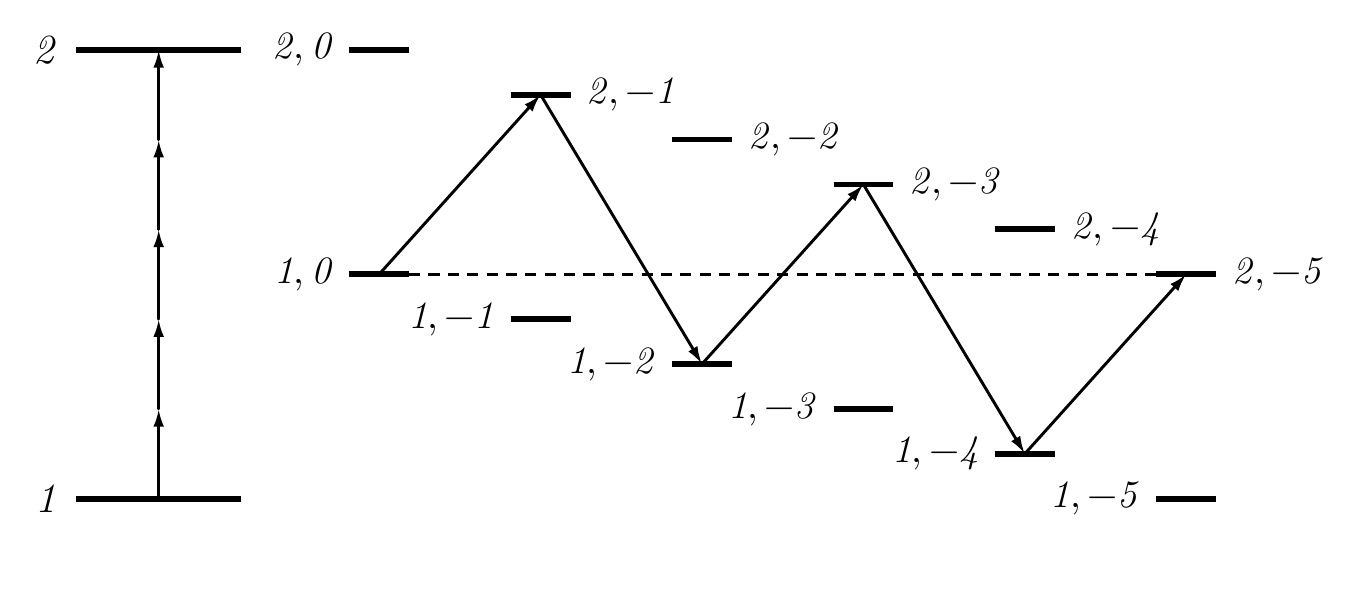
\begin{tikzpicture}[x=1cm,y=1cm]
\def\Photon{1}\def\Eone{0}\pgfmathsetmacro\Etwo{5*\Photon}
\def\BaseA{.80}\def\ScaleB{.57}
\pgfmathsetmacro\ScaleA{2*\ScaleB}
\pgfmathsetmacro\BaseB{\BaseA+5*\ScaleB}
\def\Xzero{4.35}\def\DX{2.05}
\def\HalfLevel{.38}\def\LabelGap{.13}
% a: five equal photon steps. Common top/bottom extent with panel b.
\coordinate (A1) at (1.55,\BaseA);
\coordinate (A2) at (1.55,{\BaseA+\ScaleA*\Etwo});
\draw[level] ($(A1)+(-1.05,0)$)--($(A1)+(1.05,0)$);
\draw[level] ($(A2)+(-1.05,0)$)--($(A2)+(1.05,0)$);
\node[lab,anchor=east] at ($(A1)+(-1.22,0)$) {$\mathit{1}$};
\node[lab,anchor=east] at ($(A2)+(-1.22,0)$) {$\mathit{2}$};
\foreach \k in {0,...,4}{
 \draw[photon] (1.55,{\BaseA+\k*\ScaleA*\Photon})--(1.55,{\BaseA+(\k+1)*\ScaleA*\Photon});
}
% b: both complete replica families, with coordinates determined only by En and K.
\foreach \k in {0,...,5}{
 \pgfmathsetmacro\xc{\Xzero+\k*\DX}
 \pgfmathsetmacro\lo{\BaseB+\ScaleB*(\Eone-\k*\Photon)}
 \pgfmathsetmacro\hi{\BaseB+\ScaleB*(\Etwo-\k*\Photon)}
 \coordinate (L\k) at (\xc,\lo); \coordinate (U\k) at (\xc,\hi);
 \coordinate (L\k left) at ($(L\k)+(-\HalfLevel,0)$);
 \coordinate (U\k left) at ($(U\k)+(-\HalfLevel,0)$);
 \draw[level] (L\k left)--($(L\k)+(\HalfLevel,0)$);
 \draw[level] (U\k left)--($(U\k)+(\HalfLevel,0)$);
}
% Draw the resonant horizontal guide only in open intervals, not through 1,0 or 2,-5.

\foreach \from/\to in {L0/U1,U1/L2,L2/U3,U3/L4,L4/U5}{
 \draw[photon] (\from)--(\to);
}
% State labels: upper family on the right, lower family on the left, at level height.
% k=0 remains in the left margin, matching the original figure.
\foreach \k in {0,...,5}{
 \ifnum\k=0
  \node[levlab,anchor=east] (Ulabel\k) at ($(U\k left)+(-\LabelGap,0)$) {$\mathit{2,0}$};
  \node[levlab,anchor=east] (Llabel\k) at ($(L\k left)+(-\LabelGap,0)$) {$\mathit{1,0}$};
 \else
  \node[levlab,anchor=west] (Ulabel\k) at ($(U\k)+(\HalfLevel+\LabelGap,0)$) {$\mathit{2,-\k}$};
  \node[levlab,anchor=east] (Llabel\k) at ($(L\k left)+(-\LabelGap,0)$) {$\mathit{1,-\k}$};
 \fi
}
% The guide joins level endpoints. The final-state label is now outside it, on the right.
\draw[virtual] ($(L0)+(\HalfLevel,0)$)--($(U5)+(-\HalfLevel,0)$);
\node[panel] at (1.55,.00) {а};
\node[panel] at ({\Xzero+2.5*\DX},.00) {б};
\end{tikzpicture}

\end{document}
